\documentclass[tikz]{standalone}
\usepackage{amsmath,amssymb}
\usetikzlibrary{arrows.meta}

% Classes of morphisms
\newcommand{\all}{\mathsf{all}}
\newcommand{\inj}{\mathsf{inj}}
\newcommand{\surj}{\mathsf{surj}}
\newcommand{\bij}{\mathsf{bij}}
\newcommand{\init}{\mathsf{init}}
\newcommand{\pb}{\mathsf{pb}}
\newcommand{\homog}{\mathsf{homog}}
\DeclareMathOperator{\id}{id}
\renewcommand\emptyset\varnothing
\begin{document}
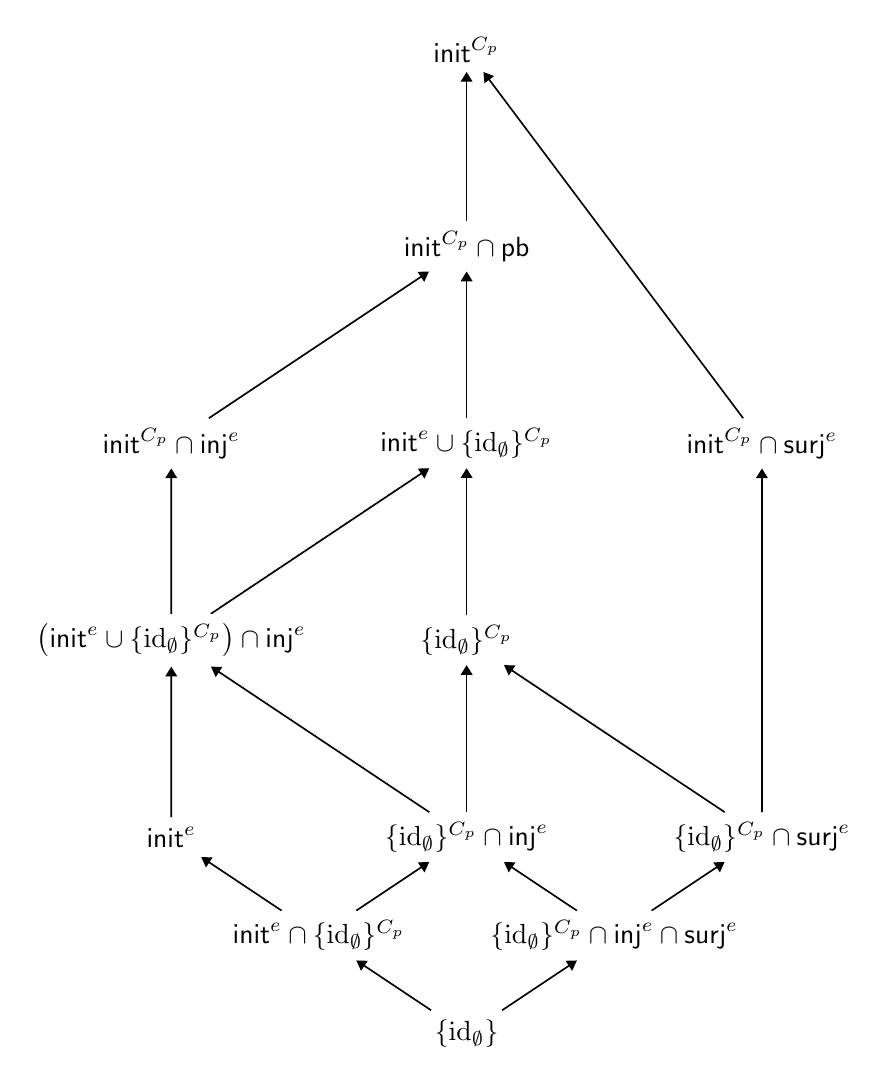
\begin{tikzpicture}[scale=2.5]
    \node (v0) at (0, -2) {$ \{\id_\emptyset\} $};
    \node (v1) at (-1.5, -1) {$ \init^e $};
    \node (v2) at (-0.75, -1.5) {$ \init^e \cap \{\id_\emptyset\}^{C_p} $};
    \node (v3) at (0, 0) {$ \{\id_\emptyset\}^{C_p} $};
    \node (v4) at (0, 1) {$ \init^e \cup \{\id_\emptyset\}^{C_p} $};
    \node (v5) at (0, 2) {$ \init^{C_p} \cap \pb $};
    \node (v6) at (0, 3) {$ \init^{C_p} $};
    \node (v7) at (1.5, -1) {$ \{\id_\emptyset\}^{C_p} \cap \surj^e $};
    \node (v8) at (1.5, 1) {$ \init^{C_p} \cap \surj^e $};
    \node (v9) at (0, -1) {$ \{\id_\emptyset\}^{C_p} \cap \inj^e $};
    \node (v10) at (-1.5, 0) {$ \left(\init^e \cup \{\id_\emptyset\}^{C_p}\right) \cap \inj^e $};
    \node (v11) at (-1.5, 1) {$ \init^{C_p} \cap \inj^e $};
    \node (v12) at (0.75, -1.5) {$ \{\id_\emptyset\}^{C_p} \cap \inj^e \cap \surj^e $};
    \draw[white, ultra thick, double=black, arrows={-Triangle[black,scale=0.25]}] (v0) -- (v2);
    \draw[white, ultra thick, double=black, arrows={-Triangle[black,scale=0.25]}] (v0) -- (v12);
    \draw[white, ultra thick, double=black, arrows={-Triangle[black,scale=0.25]}] (v2) -- (v1);
    \draw[white, ultra thick, double=black, arrows={-Triangle[black,scale=0.25]}] (v2) -- (v9);
    \draw[white, ultra thick, double=black, arrows={-Triangle[black,scale=0.25]}] (v1) -- (v10);
    \draw[white, ultra thick, double=black, arrows={-Triangle[black,scale=0.25]}] (v12) -- (v7);
    \draw[white, ultra thick, double=black, arrows={-Triangle[black,scale=0.25]}] (v12) -- (v9);
    \draw[white, ultra thick, double=black, arrows={-Triangle[black,scale=0.25]}] (v7) -- (v8);
    \draw[white, ultra thick, double=black, arrows={-Triangle[black,scale=0.25]}] (v7) -- (v3);
    \draw[white, ultra thick, double=black, arrows={-Triangle[black,scale=0.25]}] (v8) -- (v6);
    \draw[white, ultra thick, double=black, arrows={-Triangle[black,scale=0.25]}] (v9) -- (v3);
    \draw[white, ultra thick, double=black, arrows={-Triangle[black,scale=0.25]}] (v9) -- (v10);
    \draw[white, ultra thick, double=black, arrows={-Triangle[black,scale=0.25]}] (v3) -- (v4);
    \draw[white, ultra thick, double=black, arrows={-Triangle[black,scale=0.25]}] (v10) -- (v4);
    \draw[white, ultra thick, double=black, arrows={-Triangle[black,scale=0.25]}] (v10) -- (v11);
    \draw[white, ultra thick, double=black, arrows={-Triangle[black,scale=0.25]}] (v4) -- (v5);
    \draw[white, ultra thick, double=black, arrows={-Triangle[black,scale=0.25]}] (v11) -- (v5);
    \draw[white, ultra thick, double=black, arrows={-Triangle[black,scale=0.25]}] (v5) -- (v6);
    \node[fill=white] at (v0) {$ \{\id_\emptyset\} $};
    \node[fill=white] at (v1) {$ \init^e $};
    \node[fill=white] at (v2) {$ \init^e \cap \{\id_\emptyset\}^{C_p} $};
    \node[fill=white] at (v3) {$ \{\id_\emptyset\}^{C_p} $};
    \node[fill=white] at (v4) {$ \init^e \cup \{\id_\emptyset\}^{C_p} $};
    \node[fill=white] at (v5) {$ \init^{C_p} \cap \pb $};
    \node[fill=white] at (v6) {$ \init^{C_p} $};
    \node[fill=white] at (v7) {$ \{\id_\emptyset\}^{C_p} \cap \surj^e $};
    \node[fill=white] at (v8) {$ \init^{C_p} \cap \surj^e $};
    \node[fill=white] at (v9) {$ \{\id_\emptyset\}^{C_p} \cap \inj^e $};
    \node[fill=white] at (v10) {$ \left(\init^e \cup \{\id_\emptyset\}^{C_p}\right) \cap \inj^e $};
    \node[fill=white] at (v11) {$ \init^{C_p} \cap \inj^e $};
    \node[fill=white] at (v12) {$ \{\id_\emptyset\}^{C_p} \cap \inj^e \cap \surj^e $};
\end{tikzpicture}
\end{document}